\documentclass[serif,notheorems]{beamer}
\usetheme{Berlin}
\usecolortheme{seagull}
\usepackage[utf8]{inputenc}
\usepackage[T1]{fontenc}
\usepackage{csvsimple}
\usepackage{graphicx}
\usepackage{verbatim}
\usepackage{sansmathaccent}
\pdfmapfile{+sansmathaccent.map}
\usepackage{amsmath,mathtools}

% immmagini
\graphicspath{ {./img/} } % Path relative to the main .tex file 
\usepackage[labelformat=empty]{caption}

% per inserire immagini:
%\begin{figure}[H]
%\centering
%\includegraphics[scale=.8]{Images/EM on elliptic data %3.png}
%\caption{E-M on elliptic data, 3 clusters}
%\end{figure}

% STUTTURE FONDAMENTALI
% ipotesi
\newenvironment{ipotesi}%
{\quad\left|\quad\def\arraystretch{1.2}\begin{array}{@{}l@{}}}%
{\end{array}\right.}
% tesi
\newcommand{\tesi}[1]{\quad\left|\quad{#1}\right.}
% unico comando per ipotesi e tesi
\newcommand{\hpth}[2]
{
\begin{align*}
\quad
\text{Hp}
&\begin{ipotesi}
#1
\end{ipotesi}\\
\text{Ts}
&\begin{ipotesi}
#2
\end{ipotesi}
\end{align*}
}
% quando si vuole inserire l'idea della dimostrazione
\newcommand{\hpthdim}[3]
{
\begin{align*}
\quad
\text{Hp}
&\begin{ipotesi} 
#1
\end{ipotesi}\\
\text{Ts}
&\begin{ipotesi}
#2
\end{ipotesi}\\
\text{Proof}
&\begin{ipotesi}
#3
\end{ipotesi}
\end{align*}
}
% teoremi, definizoni, dimostrazioni, osservazioni
\setbeamertemplate{theorems}[numbered] % to number
\theoremstyle{definition} % insert bellow all blocks you want in normal text
\newtheorem{theorem}{Teorema}[section] % to number according to section
\newtheorem{definition}{Definizione}[section] % to number according to section
\newtheorem*{idea}{Idea dimostrazione} % no numbered block
\theoremstyle{remark}
\newtheorem*{remark}{Osservazione}


% NOTAZIONE
% sistemi
\newenvironment{system}%
{\left\lbrace\begin{array}{@{}l@{}}}%
{\end{array}\right.}
% parte intera
\newcommand{\interior}[1]{\accentset{\circ}{#1}}
% norma
\newcommand\norm[1]{\left\lVert#1\right\rVert}
% absolute value
\newcommand\abs[1]{\left|#1\right|}


% FUNZIONAMENTO MATRICI
\makeatletter
\renewcommand*\env@matrix[1][*\c@MaxMatrixCols c]{%
  \hskip -\arraycolsep
  \let\@ifnextchar\new@ifnextchar
  \array{#1}}
\makeatother





\title{ The Cauchy-Kowalevski Theorem \\ and Its Consequences }
\author{Candidate: Alessandro Pedone,\\ Advisor: Prof. Maurizio Grasselli }
\institute{Politecnico di Milano}
\date{24 september 2024}

\begin{document}

\frame{\titlepage}
\begin{frame}
    \frametitle{Indice}
    \tableofcontents
\end{frame}


\section{Introduction}

\begin{frame}
\frametitle{Sofya Vasilyevna Kovalevskaya (1850-1891)}
We assume the historical figure of Augustin-Louis Cauchy is well-known. \\
Kowalevski was:
\begin{itemize}
\item a Russian mathematician and student of Weierstrass
\item the \textbf{first woman} to earn a doctorate (3 theses dating back to 1875) and to obtain a chair in Europe (in mathematics)
\end{itemize}
\end{frame}

\begin{frame}
There are several \textbf{artistic representations} of her in both literature and cinema. The most notable are:
\begin{itemize}
\item An accurate biography: \textit{Little Sparrow: A Portrait of Sophia Kovalevsky} (1983), Don H. Kennedy
\item A short story: \textit{Too Much Happiness} (2009), Alice Munro
\end{itemize}
\end{frame}


\begin{frame}
\frametitle{Guiding Questions}
\begin{center}
\textit{ Is it possible for an analytical solution \\ of a PDE system \\ with Cauchy conditions to exist?}
\end{center}
\end{frame}

\begin{frame}
The answer is affirmative, so we already ask:
\begin{itemize}
\item under what assumptions?
\item is the solution unique?
\item is the problem well-posed?
\item what are the consequences of the obtained results?
\end{itemize}
\end{frame}

\section{Fundamental Tools}

\begin{frame}
\frametitle{Types of Equations (and Operators)}
Equations of order $k$:
\begin{table}
\renewcommand{\arraystretch}{2}
\begin{tabular}{l l} 
\hline \hline
 Linear & $\sum_{|\alpha |\leq k} a_\alpha \, D^\alpha u = f$ \\
 \hline
 \vspace{-2mm}
 Quasi-linear & $\sum_{|\alpha |= k} a_\alpha (x,D^\beta u) \, D^\alpha u +  a_0(x,D^\beta u)= f,$\\
 & $\quad |\beta |<k $ \\
 \hline
 Non-linear & $F(x,D^\alpha u)=0, \quad |\alpha | \leq k$ \\
 \hline
 In normal form & $D_{t}^k u = G(x, D^\alpha_x D^j_t u), \quad |\alpha |+j \leq k, \, j < k$ \\
 \hline \hline
\end{tabular}
\end{table}
\end{frame}

\begin{frame}
\frametitle{Tools}
\begin{itemize}
\item Characteristic surfaces
\item Method of characteristics
\item Cauchy problems
\item Power series
\end{itemize}
\end{frame}

\begin{frame}
\frametitle{Characteristic Surfaces for Linear Operators}
$L$ linear differential operator.
\begin{definition}
Characteristic form of $L$:\\ $\chi_L(x,\xi)=\sum\limits_{|\alpha |= k} a_\alpha(x) \, \xi^\alpha \quad \text{with} \quad x,\xi \in \mathbb{R}^n$
\end{definition}

\begin{definition}
Characteristic variety of $L$ at $x$:\\ $\text{char}_x (L)= \{ \xi \neq 0 : \chi_L(x,\xi)=0 \}$
\end{definition}
\end{frame}

\begin{frame}
\begin{definition}
$\Gamma$ characteristic surface for $L$ at $x \iff \nu(x) \in\text{char}_x (L)$
\end{definition}
\begin{remark}
Case of 1st order operator: $A=(a_1,\ldots ,a_n)$ tangent to $\Gamma$.\\
Useful for further generalizations.
\end{remark}
\end{frame}

\begin{frame}
\frametitle{Meaning}
$$\xi \in \text{char}_x (L)$$
at $x$ $L$ is not ``properly'' of order $k$ in the direction $\xi$.
\vspace{5mm}
$$\Gamma \text{ non-characteristic }$$ 
given $D^i_\nu u \,(i<k)$ of a solution $u$ on $\Gamma$
it is possible to calculate all its partial derivatives on $\Gamma$.
\end{frame}

\begin{frame}
\frametitle{1st Order Quasi-linear Operators}
\begin{itemize}
\item $\gamma (s): \mathbb{R}^{n-1}\rightarrow \mathbb{R}^n$ local parametrization of $\Gamma$
\item $u = \phi$ on $\Gamma$ Cauchy data
\end{itemize}
\begin{definition}
$\Gamma$ non-characteristic at $x_0=\gamma (s_0)$\\
\begin{equation*}
\iff \det
\underbrace{
\left[
\begin{matrix}
D_{s_1}\gamma_1 & \cdots & D_{s_{n-1}}\gamma_1 \\
\vdots &  & \vdots \\
D_{s_1}\gamma_n & \cdots & D_{s_{n-1}}\gamma_n \\
\end{matrix}\;\right|}_{\text{span of the tangent plane}} \,
\left.
\begin{matrix}
a_1(\gamma, \phi(\gamma))\\
\vdots\\
a_n(\gamma, \phi(\gamma))\\
\end{matrix}\right] (s_0) \neq 0
\end{equation*}
\end{definition}
\end{frame}

\begin{frame}
\frametitle{Method of Characteristics}
The following problems\footnote{it can be generalized to the nonlinear case (1st order!)} are \textbf{equivalent}.
\begin{equation} \label{edpquasilin}
PDE:
\begin{cases}
\sum a_j(x,u)D_{x_j} u = b(x,u)\\
u = \phi \text{ on } \Gamma
\end{cases} 
\end{equation}
\begin{equation}
ODE:
\begin{cases}
D_t \, x = A(x,y) \; \footnotemark \\
D_t \, y = b(x,y)\\ 
x(0)=x_0\\ 
y(0) = \phi (x_0) \quad \forall x_0 \in \Gamma
\end{cases} 
\end{equation}
Where $y = u(x)$ and $A(x,y)=[a_1(x,y),\ldots ,a_n(x,y)]$.
\footnotetext{the solutions $x$ are called \textit{characteristic curves}}
\end{frame}

\begin{frame}
\begin{theorem}
\hpthdim{
\text{Problem \eqref{edpquasilin} } \\
a_j, \, b, \, \phi , \, \Gamma \in C^1\\
\Gamma \text{ non-characteristic}
}{
\exists ! \text{ unique } C^1 \text{ solution in a neighborhood of } \Gamma
}
{
\text{using the local existence}\\ \text{and uniqueness theorem for ODEs}
}
\end{theorem}
\end{frame}

\begin{frame}
\frametitle{Cauchy Problem}
\begin{itemize}
\item Often used when the data surface is \textbf{not} a boundary.
\item It also requires the \textbf{normal derivatives} ($D^j_\nu u$) of the solution on the surface to uniquely determine it.
\item It carries the risk of being \textbf{overdetermined} (good for uniqueness but less for the existence of the solution).
\end{itemize}
\end{frame}

\begin{frame}
\frametitle{General Problem}
\begin{equation*}
\begin{cases}
F^*(x,D^\alpha u^*)=0 & |\alpha | \leq k, \, F^* \text{ at least } C^1\\
D^j_\nu u^* = \phi_j^* & \text{on } \Gamma^* \text{ for }j<k 
\end{cases}
\end{equation*}
\end{frame}

\begin{frame}
\frametitle{Mapping at $t=0$}
Let $\gamma^*$ be the local parametrization of $\Gamma^*$, we apply the map:
$$\Phi (x) = 
\begin{bmatrix}[ccc|c]
x_1 & \cdots & x_{n-1} & x_n-\gamma^* (x_1,\ldots , x_{n-1})
\end{bmatrix}$$
\begin{figure}[H]
\centering
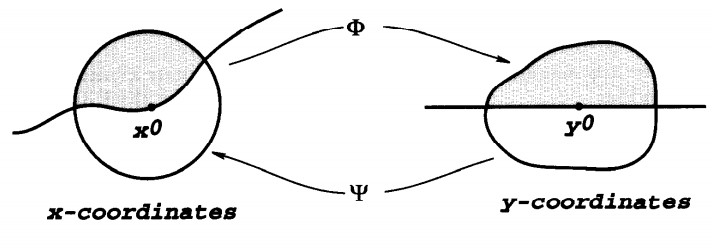
\includegraphics[scale=.35]{flatb}
\caption{\tiny{L. C. Evans, \textit{Partial Differential Equations}}}
\end{figure}
\end{frame}

\begin{frame}
\begin{enumerate}
\item Select a privileged variable and call it ``time'':
\begin{align*}
t & \leftarrow x_n \\
x & \leftarrow (x_1,\ldots , x_{n-1})
\end{align*}
\item Call $\Gamma_0 = \{t=0\}$.
\item Indicate the derivatives as follows: $D^\alpha_x D^j_t u$.
\item Obtain the problem ($u^*=u(\Phi)$):
\begin{equation*}
\begin{cases}
F(x,t, D^\alpha_x D^j_t u)=0 & |\alpha | +j \leq k\\
D^j_t u (x,0)= \phi_j(x) & \text{for }j<k 
\end{cases}
\end{equation*}
\end{enumerate}
\end{frame}

\begin{frame}
\frametitle{Non-characteristic Surfaces in General}
\begin{definition}
$\Gamma^*$ (or $\Gamma_0$) is non-characteristic $\iff$ the equation on $\Gamma_0$ can be rewritten in \textbf{normal form} with respect to $t$.
\end{definition}
\begin{remark}
It is shown to be consistent with previous definitions.
\end{remark}
\begin{remark}
\begin{itemize}
\item Linear case $\rightarrow$ condition on the coefficients.
\item Non-linear case $\rightarrow$ validity of implicit function theorem hypotheses on $F$.
\end{itemize}
\end{remark}
\end{frame}

\begin{frame}
\frametitle{Remarkable Power Series}
\begin{definition}
Majorizing function: $$\mathcal{M}_{Cr}(x)=\frac{Cr}{r-(x_1+\ldots +x_n)}$$
\end{definition}
\begin{remark}
By the multinomial theorem, if $|x|<r/n$ we have that
$$\frac{Cr}{r-(x_1+\ldots +x_n)}=C \sum\limits_\alpha \frac{|\alpha |!}{\alpha ! \, r^{|\alpha |}} x^\alpha.$$
\end{remark}
\end{frame}

\begin{frame}
\frametitle{Method of Majorants}
\begin{theorem}[utility of the majorant]
\begin{equation*}
\begin{cases}
g_\alpha \geq |f_\alpha|\\
\sum g_\alpha x^\alpha \text{ has a radius of conv. } R
\end{cases}
\implies 
\begin{array}{c}
\sum f_\alpha x^\alpha \\
\text{has a radius at least } R
\end{array}
\end{equation*}
\end{theorem}
In this case, we write: $\sum g_\alpha x^\alpha \gg \sum f_\alpha x^\alpha$.
\end{frame}

\begin{frame}
\begin{theorem}[construction of the majorant]
$\sum f_\alpha x^\alpha$ has radius $R \implies \exists \, r<R, \, C>0$ such that 
$$|f_\alpha | \leq C \frac{1}{r^{|\alpha |}} \leq C \frac{|\alpha |!}{\alpha ! \, r^{|\alpha |}}$$
\end{theorem}
\end{frame}

\section{Invariant Version}

\begin{frame}
\frametitle{Outline of the Approach}
Following the chronological order of discovery, we proceed by \textbf{progressive generalizations}:
\begin{enumerate}
\item ODEs
\item Quasi-linear PDEs
\item PDEs in normal form
\end{enumerate}
\end{frame}

\begin{frame}
\frametitle{ODE}
\begin{theorem}
\hpth{
A \subseteq \mathbb{C}, \, B\subseteq \mathbb{C}^n \text{ open }\\
\Omega \subseteq A \text{ open, connected}\\
f:A\times B\rightarrow\mathbb{C}^n \text{ holomorphic}\\
\text{Pb: }
\begin{cases}
y' = f(x,y) \quad \forall x \in \Omega \\
y(x_0)=y_0
\end{cases}\\
}
{
\text{locally there exists a unique holomorphic solution}
}
\end{theorem}
\end{frame}

\begin{frame}
\frametitle{Radius Estimate}
\begin{theorem}
\hpth{
\text{Assumptions of the previous theorem}\\
\exists \, \overline{B_a(x_0)}\subseteq A,\,\overline{B_b(y_0)} \subseteq B\\
}{
\text{The solution converges with at least radius}\footnotemark \\
\widetilde{r}= a\left[ 1-\exp\left( -\frac{b}{aM(n+1)}\right) \right] \\
}
\end{theorem}
\footnotetext{$M=\max_{B_a(x_0),\, B_b(y_0)}|f|$}
\end{frame}

\begin{frame}
\frametitle{Quasi-linear PDEs}
\begin{theorem}\label{teoquasilin}
\hpth{
A_j , \, B\text{ analytic }\\
\text{Pb: }
\begin{cases}
D_t \, y = \sum\limits_{j=1}^{n-1} A_j(x,y)D_{x_j}y+B(x,y) \; \\
y=0 \quad \text{ on } \Gamma_0
\end{cases}
\\
}{
\exists ! \; y(x,t): \mathbb{R}^n \rightarrow \mathbb{R}^m
\text{ analytic solution } \\ \text{in a neighborhood of the origin}
}
\end{theorem}
\end{frame}

\begin{frame}
\frametitle{Proof}
\begin{enumerate}
\item Assume $y_h = \sum c_h^{\alpha j} x^\alpha t^j$
\item Inserting the series of $y,\, A_j,\, B$ we get: 
$$ c_h^{\alpha j} = Q_h^{\alpha j}(\text{coeff. of series of }A_j, \, B)$$
$Q$ polynomial with non-negative coefficients
\item $\widetilde{A}_i \gg A_i, \, \widetilde{B} \gg B \implies \widetilde{y} \gg y$ thanks to $Q$
\item Choose $\widetilde{A}_i, \, \widetilde{B}$ so that $\widetilde{y}$ can be explicitly calculated as analytic with the method of characteristics
\end{enumerate}
\end{frame}

\begin{frame}
\frametitle{Majorizing System}
As we already know, we majorize the series with 
$$\mathcal{M}_{Cr}(x,y) \gg A_j,\, B$$
and solve the problem\footnote{with $h=1,\ldots, m$}:
\begin{equation*}
\begin{cases}
D_t \, \widetilde{y}_h = \mathcal{M}_{Cr} \left[\sum\limits_{i,\, j} D_{x_j}\widetilde{y}_i+1 \right] \\
\widetilde{y_h}=0 \quad \text{ on } \Gamma_0
\end{cases}
\end{equation*}
\end{frame}

\begin{frame}
\frametitle{Majorant Solution}
The previous system has the solution:
$$\widetilde{y}_h(x,t)=u(x_1+\cdots +x_n,\,t) \quad \forall h$$
with
$$u(s,t)=\frac{r-s-\sqrt{(r-s)^2-2tCrmn}}{mn},$$
whose radius of convergence we can study.
\end{frame}

\begin{frame}
\frametitle{Radius of Convergence Estimate}
\begin{theorem}
The solution of theorem \ref{teoquasilin} converges with radius at least
$$\widetilde{r} = \dfrac{1}{n-1}\, \dfrac{r}{8Cmn} \text{ with } C \geq \frac{1}{2}$$
\end{theorem}

Let's observe its behavior\footnote{\textit{trade-off} $Cr$} with respect to $r$, knowing that:
\begin{align*}
r <& \min \{ \textit{radii of conv. of the coefficients } a^j_{ml}, \, b_m\} \\
C \geq & \max \begin{Bmatrix}
\max\limits_{j,m,l,\alpha } \left|a^j_{ml} \, r^{|\alpha |}\right|\\
\max\limits_{m,\alpha} \left|b_m \, r^{|\alpha |}\right|
\end{Bmatrix}
\end{align*}
\end{frame}

\begin{frame}
\frametitle{PDE in Normal Form}
\begin{theorem}
The following two problems are equivalent
\begin{align*}
\text{nonlinear : }&
\begin{cases}
D_{t}^k u = G(x, D^\alpha_x D^j_t u) & |\alpha |+ j \leq k, \, j<k \\
D_t^ju = \phi_j & \text{ on } \Gamma_0, \, j<k
\end{cases} \\
\text{quasi-linear : }&
\begin{cases}
D_t \, y = \sum\limits_{j=1}^{n-1} A_j(x,y)D_{x_j}y+B(x,y) \; \\
y=0 \quad \text{ on } \Gamma_0
\end{cases}
\end{align*}
\end{theorem}
\end{frame}

\begin{frame}
\frametitle{Proof}
\begin{enumerate}
\item The system is constructed so that $y_{\alpha j}= D^\alpha_x D^j_t u$
\end{enumerate}
\end{frame}

\begin{frame}
The matrices $A_j$ and $B$ will then be derived from the expressions\footnote{$i(\alpha)=\min\{ i:\alpha\neq 0 \} $}:
\begin{align*}
D_t y_{\alpha j} =& y_{\alpha (j+1)} & |\alpha| + j < k \\
D_t y_{\alpha j} =& D_{x_i} y_{(\alpha-1_i)(j+1)} & |\alpha| + j = k, \; j < k\\
D_t y_{0k} =& D_tG + \sum_{|\alpha|+j < k} D_{y_{\alpha j}}G y_{\alpha (j+1)} \\
& + \sum_{|\alpha|+j = k, \; j < k} D_{y_{\alpha j}} G D_{x_i} y_{(\alpha-1_i)(j+1)}
\end{align*}
The Cauchy data will be:
\begin{align*}
y_{\alpha j}(x, 0) = & D_x^{\alpha} \phi_j(x) & j < k\\
y_{0k}(x, 0) = & G\left( x, 0, D_x^{\alpha} \phi_j(x) \right) & \lvert \alpha \rvert + j \leq k, \; j < k
\end{align*}
\end{frame}

\begin{frame}
\begin{enumerate}
\setcounter{enumi}{1}
\item removing $\phi$ : $y(x,t)\leftarrow y(x,t)-\phi (x)$
\item removing $t$ : the variable $y^0=t$ is added (with its corresponding equation)
\end{enumerate}
\end{frame}

\begin{frame}
\frametitle{Holomorphic Version}
\begin{center}
As in the case of ODEs, everything extends in an \textbf{immediate}\\
way to the complex case by assuming holomorphic data.
\end{center}
\end{frame}

\section{Examples}

\begin{frame}
\frametitle{Examples}
We now answer the questions with three examples:
\begin{itemize}
\item Lewy's example: importance of analyticity
\item Kowalevski's example: importance of non-characteristicity
\item Hadamard's example: the problem might not be well-posed
\end{itemize}
\end{frame}

\begin{frame}
\frametitle{Lewy's Example}
\begin{definition}
$$\mathcal{L}=D_x+iD_y-2i(x+iy)D_t$$
is called Lewy's operator.
\end{definition}
\end{frame}

\begin{frame}
\begin{theorem}
\hpthdim{
f \text{ continuous real-valued function}\\ 
\text{depending only on } \; t\\
u\in C^1\;:\;\mathcal{L}u=f \text{ in a neighborhood of the origin }
}
{f \text{ analytic in a neighborhood of } t=0}{
\text{Schwarz reflection principle}
}
\end{theorem}
\end{frame}

\begin{frame}
The previous statement can be generalized as follows:
\begin{theorem}
\hpth{
A \subseteq \mathbb{R}^3 \text{ open }\\
}
{
\exists \, F \in C^{\infty}(\mathbb{R}^3,\mathbb{R}) \; : \; \nexists \, u \in C^1(A,\mathbb{R}) \\ \text{ such that }
\begin{cases}
\mathcal{L}u=F \text{ in } A\\
\vspace{-1mm}
u_x,\,u_y,\,u_t \text{ satisfy} \\
\text {the Hölder condition }
\end{cases}
}
\end{theorem}
\end{frame}

\begin{frame}
\frametitle{Proof}
\begin{enumerate}
\item
Translate the problem of the previous theorem so as to reduce it to the case of a generic point $(x_0,y_0,t_0)$, using the function $g(x,y,t)=f(t-2xy_0+2x_0y)$ as the forcing function.
\item
Construct a function $S_a \in C^\infty$ for each $a \in l^\infty$ using a series.
\item
Construct closed sets $E_{j,n} \subseteq l^\infty$ with no interior using $S_a$ and the Ascoli-Arzelà theorem.
\item
Conclude the proof of the new theorem using the aforementioned lemmas to derive, by a contradiction argument, the equality $l^\infty = \bigcup E_{j,n}$, allowing the application of Baire's argument.
\end{enumerate}
\end{frame}

\begin{frame}
\frametitle{Kowalevski's Example} 
This problem admits no analytic solutions\footnote{proof by contradiction} in a neighborhood of the origin:
\begin{equation*}
\begin{cases}
u_t-u_{xx}=0\\
u(x,0)=\frac{1}{1+x^2} \quad \forall \, x \in \mathbb{R}
\end{cases}
\end{equation*}
\begin{remark}
The surface is characteristic!
\end{remark}
\end{frame}

\begin{frame}
\frametitle{Hadamard's Example}
\begin{equation*}
\begin{cases}
u_{xx}+u_{yy}=0\\
u(x,0)=0\\ 
u_y(x,0)=n\sin(nx)e^{-\sqrt{n}} \text{ with } n\in\mathbb{N}
\end{cases}
\end{equation*}
The solution to this problem is:
$$u_n(x,y)=\sin(nx) \underbrace{\sinh(ny)e^{-\sqrt{n}}}_{\xrightarrow{n\rightarrow\infty} \infty}$$
\end{frame}

\section{Alternative Versions}

\begin{frame}
\frametitle{Alternative Versions}
\begin{center}
\normalsize Abstract Version \\
\footnotesize\textit{(Ovsyannikov classes)}\\
\normalsize $$\big\Downarrow$$\\
\normalsize Classical Version \\
\footnotesize\textit{(similar to local existence and uniqueness for ODEs)}\\
\normalsize $$\big\Downarrow$$\\
\normalsize Invariant Version \\
\footnotesize\textit{(non-characteristic surfaces)}\\
\end{center}
\end{frame}

\begin{frame}
\frametitle{Classical Version}
\begin{theorem}
\vspace{-5mm}
\hpth{
\overline{\mathcal{O}}_0 \subseteq \mathcal{O}_1 \subseteq \mathbb{C}^n \text{ open connected bounded}\\
A_j, f, y_0 \text{ holomorphic wrt } z\\
A_j, f \text{ continuous wrt } t\\
\text{Pb:}
\begin{cases}
D_t y = \sum A_j (z,t) D_{z_j}y+A_0(z,t)y +f(z,t) \\
y(z,0)=y_0(z)
\end{cases}\\
}{
\exists \, \delta \in (0,T) : \exists !\, y \text{ solution when } |t|<T \\
- \text{holomorphic wrt } z\\
- \; C^1 \text{ wrt } t \quad \quad \quad \rightarrow (\neq \text{Holmgren})
}
\end{theorem}
\end{frame}

\section{Applications}

\begin{frame}
\frametitle{Consequences}
The consequences of this theorem can be observed in various fields, including the main ones:
\begin{itemize}
\item theory of differential equations
\item mathematical physics: emergence of numerous questions (what happens in reality if a local analytic solution exists?)
\item differential geometry
\item economic theory
\end{itemize}
\end{frame}

\begin{frame}
Impact on the theory of differential equations:
\begin{itemize}
\item refuting Weierstrass's conjecture
\item Holmgren's theorem
\item research on necessary and/or sufficient conditions for the existence of local solutions by Treves and Nirenberg
\item Hörmander's theory of linear differential operators
\end{itemize}
\end{frame}

\begin{frame}
\frametitle{Holmgren's Theorem}
Result of \textbf{uniqueness} of solutions for linear PDEs.
\begin{remark}
Cauchy-Kowalevski theorem does not exclude the existence of other solutions that are not analytic!
\end{remark}
\end{frame}

\begin{frame}
\begin{table}
\renewcommand{\arraystretch}{1.5}
\begin{tabular}{r||ccccc} 
CK & abstract & $\implies$  & classical & $\implies$ & invariant\\
&$\big\Downarrow$ &&&&\\
H & abstract & $\implies$ & classical & $\implies$ & invariant\\
\end{tabular}
\end{table}
\end{frame}

\begin{frame}
\frametitle{Abstract Version}
Any linear equation can be reduced to a \textbf{first-order system}, we focus on this case. 
\begin{theorem}
\hpth{
y \text{ distribution on } (\mathcal{O}_0 \cap \mathbb{R}^n) \times (-T,T):\\
- K\subseteq  \mathcal{O}_0 \cap \mathbb{R}^n \text{ compact: } y=0  \text{ in } \mathcal{O}_0 \cap \mathbb{R}^n \setminus K\\
- \begin{cases}
D_t y = \sum A_j (z,t) D_{z_j}y+A_0(z,t)y \\
y=0 \text{ for } t<0
\end{cases}\\
}{
y = 0 \text{ in } (\mathcal{O}_0 \cap \mathbb{R}^n) \times (-T,T) \\
}
\end{theorem}
\end{frame}

\begin{frame}
\frametitle{Classical Version}
\begin{theorem}
\hpth{
\Omega \subseteq \mathbb{R}^n \text{ open}\\
A_j \text{ analytic}\\
y\in C^1 (\Omega \times (-T,T)): \\ 
\begin{cases}
D_t y = \sum A_j (x,t) D_{x_j}y+A_0(x,t)y \\
y=0 \text{ for } t=0
\end{cases} \\
}{
y = 0 \text{ in a neighborhood of } \Omega \times \{ 0\}
}
\end{theorem}
\end{frame}

\begin{frame}
\frametitle{Proof}
It is an application of the abstract version to the function $$\widetilde{y}(x,t) = H(t) \, y(x,t),$$ 
which always satisfies a system of the same type.
\end{frame}

\begin{frame}
\frametitle{Cartan-Kähler Theorem}
A very important theorem in differential geometry:
\begin{itemize}
\item on the integrability of \textbf{exterior differential systems}
\item which is proved using the Cauchy-Kowalevski theorem
\item which has an application in the economic field (I. Ekeland, P.A. Chiappori)
\end{itemize}
\end{frame}

\begin{frame}
Quoting Ekeland regarding the paper written in $1999$ with Chiappori:\\
\begin{center}
\textit{This paper solves a basic problem in economic theory, which had remained open for \textbf{thirty years}, namely the characterization of market demand functions. The method of proof consists of reducing the problem to a system of nonlinear PDEs, for which convex solutions are sought. This is rewritten as an exterior differential system, and is solved by the Cartan-Kähler theorem, together with some algebraic manipulations to achieve \textbf{convexity}.}
\end{center}
\end{frame}

\begin{frame}
Despite the research conducted in those years
\begin{itemize}
\item wasn't guided by immediate applications
\item led to \textbf{disappointing} results compared to the expectations of Cauchy and Weierstrass
\end{itemize}
it has had a gigantic impact thanks to the understanding of solutions of PDE systems it allowed us to achieve.
\end{frame}

\begin{frame}
In conclusion, a quote about the relationship between Weierstrass and Kowalevski:\\
\begin{center}
\textit{All his life -- he had difficulty saying this, as he admitted, being always wary of too much enthusiasm -- all his life he had been waiting for such a student to come into this room. A student who would challenge him completely, who was not only capable of following the strivings of his own mind but perhaps of flying beyond them.}
\end{center}
\null\hfill --- Alice Munro, \textit{Too Much Happiness}
\end{frame}

\end{document}